\documentclass[11pt]{article}
\usepackage[utf8]{inputenc}
\usepackage{graphicx}
\usepackage{url}
\usepackage{amsmath}
\usepackage[]{algorithm2e}
\usepackage{float}


\title{
	{Computer Vision 1 - Assignment 1 \\
	Photometric Stereo \& Color Spaces}
}
\author{
Selene Baez Santamaria (10985417) - Andrea Jemmett (11162929)}
\date{\today}

\begin{document}

\maketitle


\section{Photometric Stereo}
The goal of this assignment is to use Matlab to implement the photometric stereo algorithm, which aims to recover a patch of surface from multiple pictures under different light sources.

For this implementation we assume five light sources are involved, all of them distant.
They are positioned facing the front, left-above, right-above, left-below and right-below corners of the surface showed in the images.

We created a function that is called without arguments and produces three figures, one for the surface albedo, one for the surface normals and one for the reconstructed shape.

\begin{figure}[!htp]
    \centering
    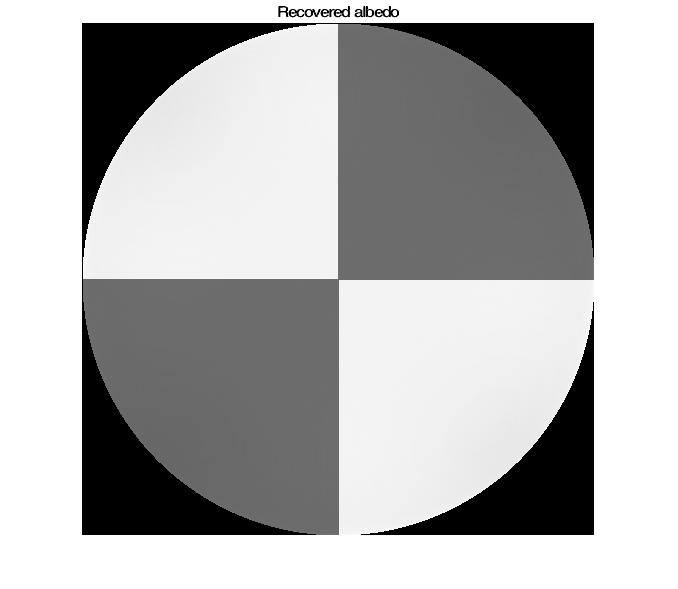
\includegraphics[width=0.4\textwidth]{albedo.jpg}
    \caption{Reconstructed albedo}
    \label{fig:albedo}
\end{figure}

Here follows a descriptions of the steps executed inside the function:
\begin{enumerate}
	\item read the given images for a sphere under different light sources and store them together in a three dimensional matrix;
	\item represent the light sources with vectors assuming a coordinate system with origin in the center of the image;
	\item \label{item:k} determine matrix $V$ from light sources. Here we introduce the scalar $k$ which controls the camera response to the input radiance;
	\item create structures to store albedo, normal, $p$ and $q$ per pixel;
	\item repeat for each pixel:
	\begin{enumerate}
		\item retrieve the pixel values for all images and store them as $i$;
		\item construct diagonal matrix $I$; 
		\item solve linear system of equations for $g$;
		\item calculate albedo, normal, $p$ and $q$;
		\item \label{item:check} derivative check to filter out big noisy values;
	\end{enumerate}
	\item show recovered albedo (e.g. in Fig. \ref{fig:albedo});
	\item show surface normals using Matlab's $quiver3$ function (e.g. in Fig. \ref{fig:normal_map});
	\item apply algorithm to reconstruct the surface height map and show it (e.g. in Fig \ref{fig:height_map}).
\end{enumerate}

Regarding the scalar $k$ used at step \ref{item:k}, we found after experimentation that a value of $100$ gives the best results.
For the derivative check at step \ref{item:check} we used a threshold of $30$ and for those pixels that don't pass the check we set $p$ and $q$ to zero.


\begin{figure}[H]
    \centering
    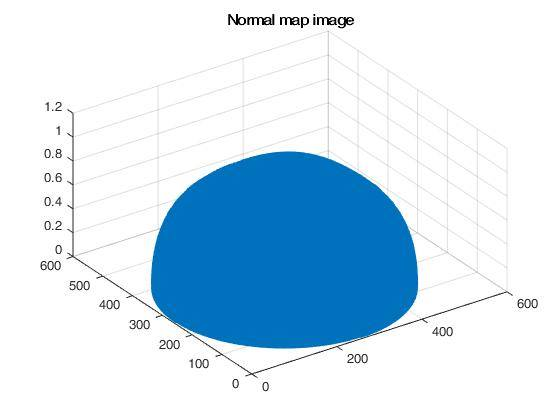
\includegraphics[width=.8\textwidth]{normals.jpg}
    \caption{Surface normals}
    \label{fig:normal_map}
\end{figure}

\begin{figure}[H]
    \centering
    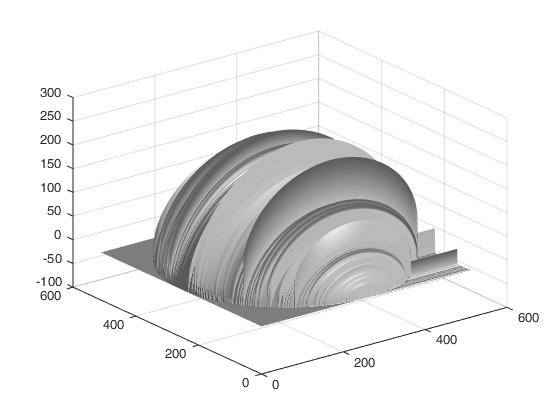
\includegraphics[width=.8\textwidth]{height_map.jpg}
    \caption{Reconstructed height map}
    \label{fig:height_map}
\end{figure}


\section{Color Spaces}
The goal of this assignment is to use Matlab to convert images between RGB and other color spaces.

We created a function that is called with two arguments: the name of the image to be converted, and the color space to be converted to.
We used the function \textit{imread} to read the image.
To compute the converted image we had to cast the 8 bits integer image (with values in the range 0 - 255) to doubles.
The converted image is then displayed as three gray-scale images (one for each channel).
We experimented with the given image “bricks.jpg” as well as other colorful images.

\subsection{Opponent Color Space}
For the RGB to \textit{Opponent} color space conversion, we used the following formula:

$$
\begin{pmatrix}
	O_1 \\
	O_2 	\\
	O_3
\end{pmatrix} = 
\begin{pmatrix}
	\frac{R - G}{\sqrt{2}}			\\
	\frac{R + G - 2B}{\sqrt{6}}		\\
	\frac{R + G + B}{\sqrt{3}}
\end{pmatrix}
$$
yielding the following image:

\begin{figure}[H]
    \centering
    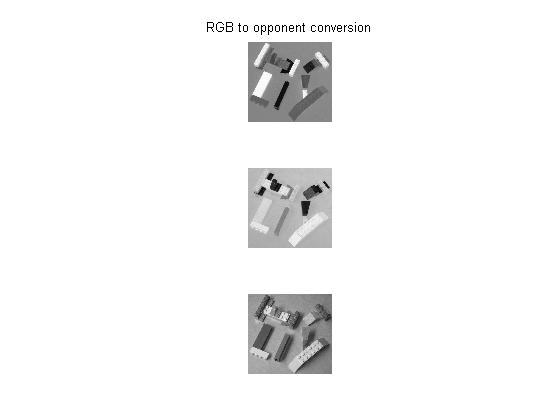
\includegraphics[width=0.8\textwidth]{bricks_to_opponent.jpg}
    \caption{RGB to Opponent Color Space}
    \label{fig:opponent_color}
\end{figure}


\subsection{rgb Color Space}
For the RGB to \textit{rgb} color space conversion, we used the following formula:

$$
\begin{pmatrix}
	r \\
	g 	\\
	b
\end{pmatrix} = 
\begin{pmatrix}
	\frac{R}{R + G + B}			\\
	\frac{G}{R + G + B}		\\
	\frac{B}{R + G + B}
\end{pmatrix}
$$
yielding the following image:

\begin{figure}[H]
    \centering
    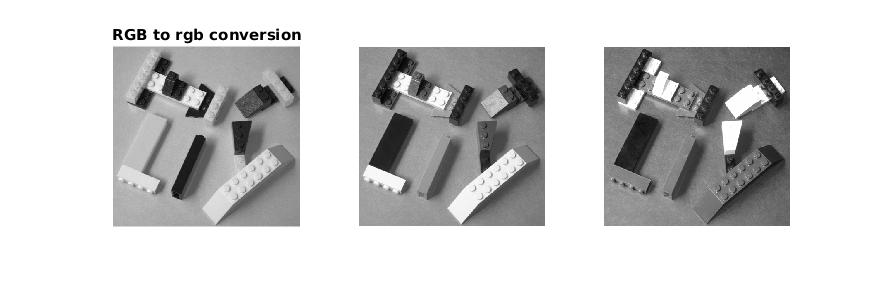
\includegraphics[width=0.8\textwidth]{bricks_to_rgb.jpg}
    \caption{RGB to rgb Color Space}
    \label{fig:rgb_color}
\end{figure}


\subsection{HSV Color Space}
For the RGB to \textit{HSV} color space conversion, we used the Matlab function \textit{rgb2hsv}, which yield the following image:

\begin{figure}[H]
    \centering
    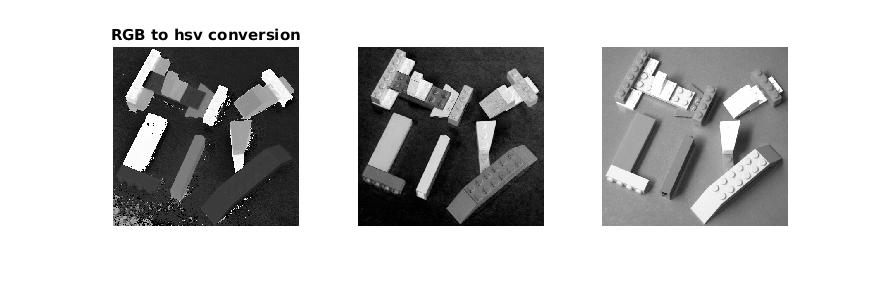
\includegraphics[width=0.8\textwidth]{bricks_to_hsv.jpg}
    \caption{RGB to HSV Color Space}
    \label{fig:hsv_color}
\end{figure}


\end{document}
